\documentclass[10pt,a4paper]{article}
\usepackage[utf8]{inputenc}
\usepackage{amsmath}
\usepackage{amsfonts}
\usepackage{amssymb}
\usepackage{makeidx}
\usepackage{graphicx}
\usepackage{float}
\usepackage{hyperref}
\hypersetup{
	colorlinks=true,
	linkcolor=blue,
	filecolor=magenta,      
	urlcolor=cyan,
}
\author{Rolando Muñoz}
\title{TgToolkit manual}

\begin{document}
\maketitle

\section{Introduction}
This plug-in focuses on TextGrid object. It is a tool for processing many annotation files in one step. Use this plug-in to create, modify, query or clean your annotation files.

\section{How to install}
To install the plug-in, (1) download the project folder from the Links section and unzip it. Then, (2) find the \textit{Praat Preference} folder. This comes by default when you use Praat for the first time. Depending on you operating system, these could be the locations:

\begin{itemize}
	\item In Linux, go to \path{/home/user name/.praat-dir}
	\item In Mac, go to \path{/Users/user name/Library/Preferences/Praat Prefs/}
	\item In Windows, go to \path{C:\Users\user name\Praat}
\end{itemize}

Now, (3) drop the project folder inside the Preferences folder. Finally, (4) open Praat. In the fixed menu, you should have \path{Praat > Goodies > tgToolkit} as in Figure \ref{fig:tgToolkit_menu}\footnote{If Praat was opened at the time you installed the plug-in, you will not see any change. So, close and open it again.}.

\begin{figure}[H]
	\centering
	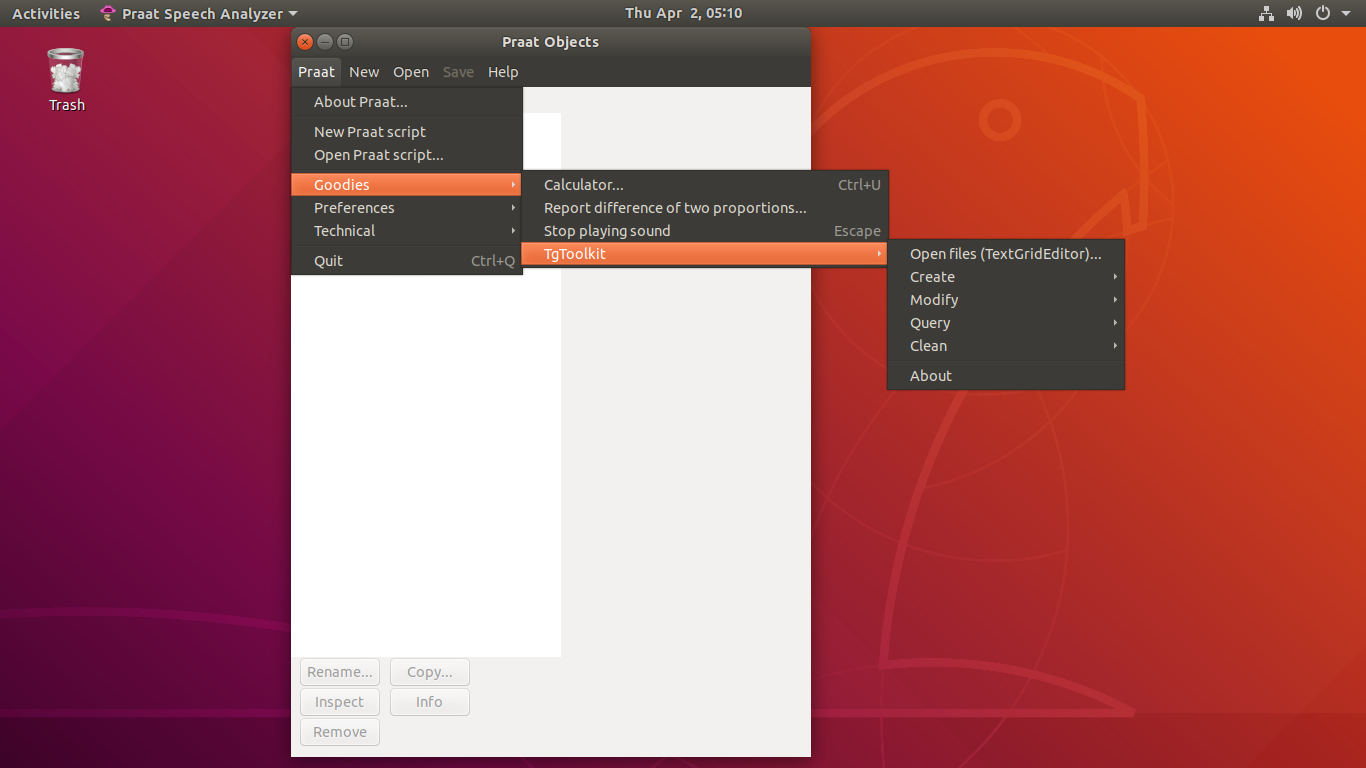
\includegraphics[scale=0.3]{img/tg_toolkit-menu}
	\label{fig:tgToolkit_menu}
	\caption{tgToolkit menu}
\end{figure}

\section{Getting started}
The \emph{tgToolkit} menu is composed of several commands. They are divided in four main categories: create, modify, query and clean. In the next sections, we will take a loot at each one.

\subsection{Create}
These commands take all the sound files stored in a directory and creates their corresponding TextGrid files. You can specify the place where to save your new files.

\subsubsection{Sound to TextGrid...}
This command is based on \href{http://www.fon.hum.uva.nl/praat/manual/Sound__To_TextGrid___.html}{Sound: To TextGrid...} It creates and saves a TextGrid file for every audio file in a directory. If a TextGrid already exists for an audio file, this command will skip that case.

\begin{figure}[H]
	\centering
	\label{fig:sound2tg}
	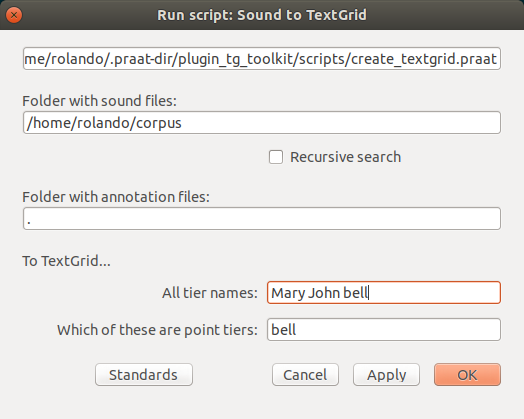
\includegraphics[scale=0.5]{img/sound2tg}
	\caption{Sound to TextGrid}
\end{figure}

\subsubsection{Sound to TextGrid (silences)...}
This command is based on \href{http://www.fon.hum.uva.nl/praat/manual/Sound__To_TextGrid__silences____.html}{Sound: To TextGrid (silences)...} It creates and saves a TextGrid file for every audio file in a directory. If a TextGrid already exists for an audio file, this command will skip that case.

\begin{figure}[H]
	\centering
	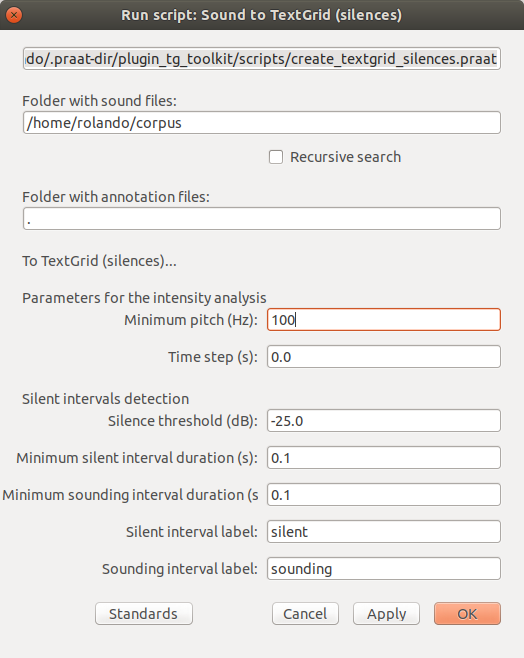
\includegraphics[scale=0.5]{img/sound2tg_silences}
	\label{fig:sound2tg_silences}
	\caption{Sound to TextGrid (silences)...}
\end{figure}

\subsection{Modify}
This set of commands modify/rewrite the TextGrid files stored in a directory.

\subsubsection{Convert}
Use this command to convert backslash tripgraphs to Unicode and vice versa.

\subsubsection{Insert tier (special)}
Use this command to insert one or more tiers in a existing TextGrid file. You can also rearrange your TextGrid tiers.

\begin{figure}[H]
	\centering
	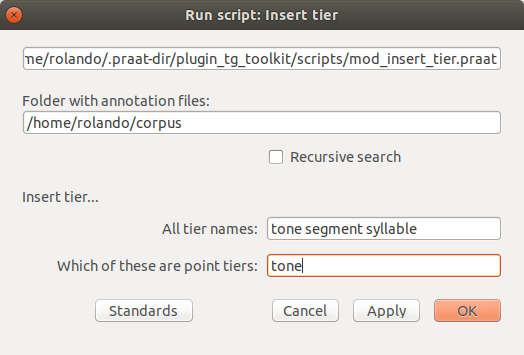
\includegraphics[scale=0.5]{img/mod_insert_tier}
	\label{fig:insert_tier}
	\caption{Insert tier...}
\end{figure}

\paragraph{Insert one or more tiers}
Enter the name of the tiers that you want to insert in \emph{All tier names}. Use blank spaces to separate between two or more tier levels. By default, this command insert only interval tiers. To insert a point tier, copy the name of the tier twice, one in \emph{All tier names} field and the other in \emph{Which of these are point tiers}. If a tier already exists in a TextGrid file, it will not be inserted.\\
Any new tier will be positioned at the top of the TextGrid layout by default. You can change this behavior and insert a new tier just below an existing tier. Include the name of that existing tier at the beginning of the list in \emph{All tier names}. By doing so, the command will first search for the position of the existing tier. Then, it will place the other tiers just below it. 

\paragraph{Rearrange tiers}
You can also use the \emph{Insert tier} command to rearrange all the existing tiers in a TextGrid. Go to \emph{All tier names} and write a list of the existing tiers in the order you want to obtained. Then, run the command. If any TextGrid layout have a different order than in the tier list, it will be rearranged.

\subsubsection{Duplicate tier}
This command is based on \emph{TextGrid: Duplicate tier...}. 
\subsubsection{Remove tier}
\subsubsection{Set tier}
\subsubsection{Replace text}
\subsubsection{Replace text (dictionary)}


\subsection{Query}
\subsubsection{Get info from annotation files}
Report TextGrid templates
\subsubsection{Find annotation files with}
\subsubsection{Report duration}
\subsection{Clean}
When working with annotation files, it gets easy to make mistakes. Some mistakes are related to 

\end{document}